\documentclass[12pt,a4paper]{report}

\usepackage[left=3cm,right=2.5cm,top=2.5cm,bottom=2.5cm]{geometry}
\usepackage{microtype}
\usepackage[euler]{textgreek}
\usepackage{hyperref}
\usepackage[backend=biber,sorting=none,backref=true]{biblatex}

% using Times Roman as default font (times package is declared obsolete):
\usepackage{newtxtext}

\usepackage{graphicx}
\graphicspath{ {./images/} }
\usepackage{subcaption} % for subfigures

% head & foot
%\usepackage{fancyhdr}

% spacing:
\linespread{1.5}

\addbibresource{sampleThesisBalintD.bib}

\title{Patch-clamp automation overview and database system development}
\author{Bálint Décsi}
%\address{Department of Biotechnology, University of Szeged}
\date{\today}

\begin{document}

\maketitle

% \begin{center}
% \vspace*{0.4cm}
% {\Large\bf University of Szeged}

% % \vspace{0.33cm}

% {\Large\bf Department of Biotechnology}

% \vspace*{2.0cm}


% {\LARGE\bf Patch-clamp automation \\ and its data structuring}


% \vspace*{1.8cm}

% {\Large Thesis sample}
% vagy {\Large Szakdolgozat}

% \vspace*{1.5cm}

% {\large \emph{Written by:} \\
%   \bf{Décsi, Bálint} \\
% }{\large Molecular Bionic Engineering\\ BSc student}

% \vspace*{1.6cm}

%Értelemszerûen megváltoztatandó:
% {\large
% \begin{tabular}{c@{\hspace{3cm}}c}
%  \multicolumn{2}{c}{\emph{Supervisors:}}\\
% \bf{G\'{a}bor R\'{a}khely, PhD Habil}  &\bf{name}\\
% Head of Department    &position\\
% Department of Biotechnology &institute\\
% University of Szeged   &Szeged\\

% \end{tabular}
% }

% \vspace*{1cm}

% {\Large
% Szeged, 2020
% }
% \end{center}

%A \chapter* parancs nem ad a fejezetnek sorszámot
% \chapter*{Task}
%A tartalomjegyzékben mégis szerepeltetni kell, mint szakasz(section) szerepeljen:
% \addcontentsline{toc}{section}{Task}

\begin{abstract}
% \addcontentsline{toc}{section}{Abstract}
My thesis aims to give a detailed overview of the evolution of patch-clamp automation techniques, focusing on recent developments in the last decade. The state-of-the-art researches in this field are structured on image-based solutions. Furthermore, I describe the plug-ins I developed for a patch-clamp automation software (Autopatcher), which are designed to visualize data collected by the software and pipeline them into a database where it can be requested from later.

% Detailing how autopatching developed from 2012 to nowadays, the main milestones (e.g. first image-guided software) and how the functionality of the plug-ins}
\end{abstract}

\tableofcontents

\chapter*{List of abbreviations}
% only if needed

\chapter{Introduction}
% \addcontentsline{toc}{section}{Introduction}

% what is electrophysiology and how the mammalian brain works:
The mammalian brain's activity consists of ionic and electrical currents occurring between specialized cells called neurons. These stimuli start from one point of the membrane of these cells and propagate towards the regions where it can be transferred to the neighboring cell. On these sites (dendrites) the neuron's signal jumps to the subsequent neuron's axon in the form of chemical (by synaptic vesicles) or electrical synapse (through gap junction). In this way, the brain can perform computations that define one's behavior. Electrophysiology is the discipline of studying this neuronal activity measuring local field potentials, the flow of the stimulus through transmembrane ion channels, calcium spikes and action potentials.\par
The greatest barrier in the performance of these measurements is the scale of the length of these currents regarding their time. They last no longer than milliseconds and for getting dependable information out of these signals, a very precise and advanced technique is necessary. Imaging methods and sensor proteins are not developed enough to be solely relied on, this is one of the reasons why patch-clamping is still the gold-standard technique for recording signals of neurons. The other reason is its relatively simple procedure. Furthermore, the previously mentioned methods can't be applied for depths of more than a few hundred microns, while patch-clamping is apt for reaching neurons in deeper brain regions, such as the thalamus.\par
% starting from the main idea of patch clamping (Neher and Sakmann, 1976), what it is for and its relevance in neurobiology:
The first reported appliance of patch-clamping was by Erwin Neher and Bert Sakmann in 1976. During their experiment they managed to measure action potentials on the membranes of individual neurons in frog thigh muscle. They lowered a fire-polished pipette of a diameter of 3--5~\textmu m onto the enzymatically cleaned membrane and held it pressed against the surface to form an electrical seal of 2--5~M\textOmega~\cite{neher1976}. By this way, it is possible to monitor the ionic current of even one transmembrane channel and get high-resolution data regarding the propagation of the stimulus. Later it was discovered that the quality of the recorded data can be improved by a slight suction in the pipette applied when it is held onto the membrane, forming a much higher seal, on the scale of gigaohms. This was baptized "gigaseal"~\cite{hamill1981} and is still referenced by that name.
% describing configurations (whole-cell, etc.):
By attaining this high magnitude of sealing, different patch-clamping configurations became achievable which were first communicated by Hamill et al. and can be seen in Fig.~\ref{fig:pcconfigs}.
\begin{figure}
    \centering
    \includegraphics[height=.4\textheight,keepaspectratio]{patchclampconfigs.png}
    \caption{Different configurations of cell-patching~\cite{hamill1981}.}
    \label{fig:pcconfigs}
\end{figure}
Once the pipette tip reached the cell surface, there are two ways to continue:
\begin{itemize}
    \item Going forward without alternating the pressure and measuring in cell-attached or inside-out state.
    \item Applying suction and conduct the measurement towards whole-cell or outside-out configuration.
\end{itemize}
% maybe will include perforated and loose patch?
In the case of cell-attached and whole-cell patch-clamping, information corresponding to the whole cell can be received. This type of experiment has the advantages of not (dramatically) perturbing the body of the cell and being able to observe ion currents of different channels and thus estimating more complex living phenomena of the neuron in focus. The other two configurations are convenient for narrowing the study on one single ion channel. In these workflows a patch of membrane is ruptured from the membrane. The inside-out method, with the cytoplasmic membrane face exposed to the bath solution (the medium in which the cell can be found) and the outside-out method, with the extracellular membrane face exposed to the bath solution also have the advantage of being able to transport and then examine the ion channel in a separate environment.\par
% image-guided in vitro:
With these techniques, only cells with freely reachable membranes could be analyzed (i.e. in a culture dish). A few years later it was discovered that patch-clamping with certain yield can be performed in brain slices if previous cleaning of the surrounding tissue is carried out. By this way, the chance of the clogging of pipette tips or false positives is reduced. The first image-guided patch-clamp research was completed in 1993 with differential interference contrast (DIC) optics and brain slices were used. With the microscopy image's feedback it became feasible to differentiate recordings from the soma and the dendrites~\cite{stuart1993}.\par
% in vivo patching:
At the same time, advances in \textit{in vivo} patching were emerging. This evolution solved a few problems relating \textit{in vitro} patching. When using brain slices, although synaptic connections remain intact, only individual neurons or smaller local circuits can be observed. This was a big barrier on the way towards understanding more complex brain functions, such as perception and memory and \textit{in vivo} patch-clamping removed this barrier.\par
% in vivo blind patching
The first successful \textit{in vivo} patch-clamp measurement was in 1991 and was tested in the visual cortex of anesthetized cats~\cite{pel1991}. The success was shaded by the fact that the electrical seal was incomplete (50--150~M\textOmega), thus this experiment only showed that \textit{in vivo} patching is possible and the demonstration of its real-life application arrived a decade later. In 2002 Margrie et al. achieved to get whole-cell recordings in the intact brain of awake, freely moving mice~\cite{margrie2002}. In \textit{in vivo} investigations the pipette must be lowered in the brain with a positive pressure present inside the tip in order to prevent clogging and blockage. Once the membrane has been reached (this is noticed by an increase in the pipette tip's resistance) the gigasealing and break-in is performed as described previously. Nevertheless, in blind patching the target depth can be theoretically infinite, which is a great advantage. On the other side, it is impossible to narrow the blind fashioned experiments in specific cell types due to the fact that the pipette tip encounters neurons randomly. Also, this method is biased towards results from bigger, more robust cells (e.g. pyramidal cells).\par
For further details on neuron morphology and wider appliance of the technique a solution for image-guided patch-clamp experiments was needed. To overcome the limitations of blind patching, two-photon laser microscopy technology was integrated with patch-clamping~\cite{margrie2003} and tested on fluorescently labelled brain cells of living transgenic mice. For the acquisition of the positions of the pipette tip and the target cell at the same time, the tip is filled with a dye with different emission spectrum from that of the cells. When the two image layers are stacked over each other by a computer, the relative position of the tip to the soma can be calculated (Fig.~\ref{fig:tptp}).
\begin{figure}
    \centering
    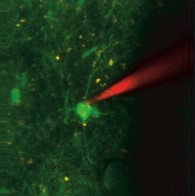
\includegraphics{tptp.jpg}
    \caption{Patch-clamping aided by dual-channel two-photon imaging~\cite{margrie2003}.}
    \label{fig:tptp}
\end{figure}
Disadvantages of \textit{in vivo} image-guided patch-clamp methodology include:
\begin{itemize}
    \item lateral movements of the tip must be limited to avoid tissue damaging,
    \item final steps of neuron hunting must be based on resistance alteration because of the depth (max. 500~\textmu m and thus the decrease in image resolution,
    \item less yield than during blind analyses.
\end{itemize}
In spite of that, it has numerous advantages which are essential for cell-type characterization and to connect morphology and neuronal function. Moreover, with the constant evolution of imaging technologies, fluorescent tags and optogenetics the number of its constraints will decrease and the possible use cases of image-guided \textit{in vivo} patch-clamping is and will be broadening.

\chapter{Automated blind patching}
% Here the content will be based on the following articles (each one from the articles that Krisztián gave me) Kodandaramaiah et al. (2012), Desai et al. (2015) and Li et al. (2017)

% weak points of human-controlled patching -> leading to importance of automation and thus scaling:
With the broadening of patch-clamping and the evolution of relating techniques, with emphasis on microscopy imaging, more and more results and advances from this area of study arose. Due to its cell-targeted usage like monitoring ion-channel-mediated events, physiological and molecular identification of cells and even manipulation of subcellular processes that define the behavior of these channels and molecules, it gained a central place in cell-type-specific neurobiology. Nevertheless, in the 2000's most of the published results from patch-clamp experiments came with a small yield and in reduced preparation, e.g. brain slices. This, on one hand, is the consequence of the fact that the performance of such experiment is labour-intensive and requires well-trained personnel. These experts have to control the pipette with \textmu m-precision, continuously change the preset values of pneumatic valves and contend with other equipment (cameras, reading values of pipette current and resistance)~\cite{desai2015}. On the other hand, a big portion of the experiments is still \textit{in vitro}, which also contributes to distortion of results, as previously mentioned (neurons remain truncated, which prohibits the acquisition of network-dependent neural responses. It could be foreseen that the focus of the upcoming researches would be on \textit{in vivo} experimenting and also that automatization of patch-clamping could solve several problems. It does not only ease the heavy load of tasks that is on the shoulders of experimenters by algorithmizing the simpler steps but also makes scaling of throughput possible.\par
% fundamental steps of patch-clamping which can be put into an algorithm:
This automation process can be seen in many methods in biology. There is a thesis that states that many techniques that evolve to be gold-standard tools in the biological sciences go through a period of transformation in which they become, at least to some degree, automated, in order to improve reproducibility, throughput and standardization~\cite{suk2019}. Patch-clamping is very often referenced as a gold-standard tool, thereby its automatization, as stated above, could be expected. There are several research groups who dedicated their attention and resources in the 2010's to the development of automated blind patch-clamp solutions. What can be observed as a common attribute of most of these investigations is the division of the whole process into four major, well-distinguishable steps (Fig.~\ref{fig:pcsteps}):
\begin{enumerate}
    \item "regional pipette localization", in which the pipette is rapidly lowered to a desired depth under positive pressure,
    \item "neuron hunting", in which the pipette is advanced more slowly at lower pressure until a neuron is detected, as reflected by a specific temporal sequence of electrode impedance changes,
    \item "gigaseal formation", in which the pipette is hyperpolarized and suction applied to create the gigaseal,
    \item "break-in", in which a brief voltage pulse (‘zap’) is applied to the cell to establish the whole-cell state.
\end{enumerate}
\begin{figure}
    \centering
    \includegraphics[width=.9\textwidth,keepaspectratio]{pcsteps.png}
    \caption{The four steps of blind patch-clamping as a skeleton for algorithms~\cite{kodandaramaiah2012}.}
    \label{fig:pcsteps}
\end{figure}

\section{Methods}
% some intro:
The first article that reports in detail a functioning automated blind patching algorithm and the hardware which it controls was that of Suhasa B Kodandaramaiah and his group, from 2012. They consequently named the robot "autopatcher"~\cite{kodandaramaiah2012}. The main feature of this rig is to divide the patching process into the four previously mentioned stages with certain pressure (p) and resistance (R) values as entry and exit criteria of these stages, with feedback system and loops. Once the break-in is successfully achieved, the ion flow measurement can start. This basic algorithm is common in several articles of the topic which were published throughout the decade.

\subsection{Flowchart overview}
The criteria dimensions p and R are picked because of the nature of the neuron hunting, gigaseal formation and break-in, which is as follows:
\begin{itemize}
    \item when lowering the pipette in the brain tissue, a small positive pressure is applied to keep the tip clean by constantly ejecting liquid (usually intracellular solution),
    \item to detect cells, pulses of electricity are delivered which diffuse in the interstitial fluid if no neuron is present in the tip's proximity,
    \item if a membrane is reached, it blocks the flow of electricity and R increases,
    \item the motion of the pipette is stopped and with a light suction (negative p) the tip gets sealed onto the membrane.
\end{itemize}
\par
The autopatcher robot is capable of recognizing these events reacting to them with minimum human intervention to get whole-cell experiment data. Its algorithm can be summarised in the flowchart in Fig~\ref{fig:flowchart}, communicated by Niraj S. Desai et al. in 2015~\cite{desai2015}.
\begin{figure}
    \centering
    \includegraphics[height=0.8\textheight,keepaspectratio]{flowchart.jpg}
    \caption{Algorithm that controls pipette lowering. The symbols P, R, and \textDelta z refer to the pressure applied to the electrode (in psi), the measured tip resistance (in M\textOmega), and incremental movement down into the brain (in \textmu m), respectively~\cite{desai2015}.}
    % convert psi into bar if having time
    \label{fig:flowchart}
\end{figure}

\subsection{Motion control}
% include Li et al. (2017)'s dodging in one of the subsections
% compare values in the diff. articles

We can declare that this component of the robot is fundamental, as this is the one that positions the pipette tip onto the membrane surface. Usually the stepper motor is preset to 200~\textmu m downwards per step, which is the initial setup once the dura mater (one of the three meninges of the brain) has been penetrated, but the alteration of its value and direction upon R-related events is often programmed into the algorithms. This value drops to 2~\textmu m during neuron hunting (or "SEARCH", in Fig.~\ref{fig:flowchart}). As stated in \cite{desai2015}, the part which is still quite complicated to automatize is lowering the pipette into the craniotomy, therefore steps involved in this movement---which are reaching the dura mater and setting initial point for z---are excluded from the algorithm.

\subsection{Regulating pressure}
% flowcharts and exact values of p depending on which state the process is in
% conclusions, i.e. what happens if standard values are changed, how clogging can be avoided via increasing p
% why is p alternating between groups: where is the balance between avoiding clogging and damaging the tissue
% could include fig. from Desai et al. (2015) "... positive and negative poles, which is added to atmospheric pressure, as can be seen on the fig."

Setting the right pressure values is essential because this is the tool for triggering several key events during the process. Its value ranges mostly between -150~mbar and 800~mbar, albeit exact quantities show considerable variance between groups and years. The main reason for this is that each experimenter has to choose between higher p during pipette localization with less chance of clogging, or lower p with less chance of harming the tissue (but greater risk of clogging). For the tuning of p is possible with a positive and negative source, a value around ±690~mbar, like in \cite{desai2015}. The logical workflow is not very complicated and can be easily overviewed by Fig.~\ref{fig:pFeedback}. The first solenoid valve determines whether positive or negative pressure would be applied. The proportional valve cuts down the magnitude of the pressure at its output. The second solenoid valve determines whether this pressure or atmospheric pressure would be piped into the pipette. An electronic pressure monitor measures the pressure output of the proportional valve and sends this number to a microcontroller ("FEEDBACK"), which compares it with the desired pressure specified by the proper software ("SET") and calculates an error equal to their difference. In overall, positive pressure is used to keep the tip clean while negative pressure is used for gigaohm sealing and for break-in (where voltage pulses are also needed). Moreover, the implementation of this algorithm worked really well as can be seen in Fig.~\ref{fig:pFeedback}, where the value set for p (by the software) and the measured feedback value does not differ throughout the experiment. This is partly due to the low temporal response secured by the PID algorithm.
\begin{figure}
    \centering
    \subcaptionbox{A schematic of the basic design. SV, solenoid valve; PV, proportional valve; P, pressure monitor; ATM, atmospheric pressure; PID, proportional-integral-derivative control algorithm; + and -, positive and negative pressure sources (10 psi). \label{flowchart}}{\includegraphics[width=.4\textwidth,keepaspectratio]{images/pFeedbackA.jpg}}
    \subcaptionbox{An example of the speed and accuracy of pressure control given by the regulator. Typical pressures for different steps in the in vivo patching process are labeled. \label{diagram}}{\includegraphics[width=.4\textwidth,keepaspectratio]{images/pFeedbackB.jpg}}
    \caption{Pressure regulation~\cite{desai2015}.}
    \label{fig:pFeedback}
\end{figure}

\subsection{Resistance monitoring}
% how the software reacts to certain values of R in certain stages of patching, (with the most detail in gigaseal formation)
% how broken pipette, blockage and neuron is recognized in diff. articles
Resistance monitoring or more generally electrode signal analysis is extremely important in blind patch-clamping since it is the only tool for detecting neurons and other "objects" in the brain, as microscopy image is absent. Its criteria values for the algorithm can be changed and adjusted, but the different groups preset certain magnitudes for them to detect events during the patch-clamping

\section{Disadvantages}
% leading the context towards image-based algorithms}
% biased towards bigger cells

% how automation appeared in image-guided processes as well

\chapter{Automated image-guided patch clamping}
% 3D rendering of stacks, two-photon vs DIC, insertion of vectors, structure-function correlation
% Also, Autopatcher, how working with it is like (though now it seems that I won’t be able to see that because of COVID-19) and leading to describing plug-ins
% Also speaking about IG patching milestones and results (with extra details in in vivo solutions)

\chapter{Data visualization and structuring of the autopatching software}
% Yet its content here depends on until where can I get with these tasks

\chapter{Conclusion}

\section{Future}
% optogenetics, nanopipettes (mentioned in Intro of 2019 article), infusion of dyes for morph-function detection and extraction of cell contents (beginning of Kondaramaiah et al., 2012)

\printbibliography

\end{document}